\documentclass[12pt]{article}
\usepackage[utf8]{inputenc}
\usepackage[spanish]{babel}
\decimalpoint
\usepackage{amsmath}
\usepackage{amsthm}
\usepackage{amssymb}
\usepackage{graphicx}
\usepackage[margin=0.9in]{geometry}
\usepackage{fancyhdr}
\usepackage[inline]{enumitem}
\usepackage{float}
\usepackage{cancel}
\usepackage{bigints}
\usepackage{color}
\usepackage{xcolor}
\usepackage{listings}
\usepackage{listingsutf8}
\usepackage{algorithm}
\usepackage{tocloft}
\usepackage[none]{hyphenat}
\usepackage{graphicx}
\usepackage{grffile}
\usepackage{tabularx}
\usepackage[nottoc,notlot,notlof]{tocbibind}
\renewcommand{\cftsecleader}{\cftdotfill{\cftdotsep}}
\pagestyle{fancy}
\setlength{\headheight}{15pt} 
\lhead{Introducción a los sistemas operativos(2)}
\rhead{\thepage}
\lfoot{Sistemas Operativos}
\renewcommand{\footrulewidth}{0.5pt}
\setlength{\parskip}{0.5em}
\newcommand{\ve}[1]{\overrightarrow{#1}}
\newcommand{\abs}[1]{\left\lvert #1 \right\lvert}

\definecolor{pblue}{rgb}{0.13,0.13,1}
\definecolor{pgreen}{rgb}{0,0.5,0}
\definecolor{pred}{rgb}{0.9,0,0}
\definecolor{pgrey}{rgb}{0.46,0.45,0.48}
\lstset{tabsize=1}

\newcommand{\tabitem}{~~\llap{\textbullet}~~}
\newcommand{\subtabitem}{~~~~\llap{\textbullet}~~}

\bibliographystyle{IEEEtran}
\usepackage{listings}
\lstdefinestyle{customc}{
  belowcaptionskip=1\baselineskip,
  breaklines=true,
  frame=L,
  xleftmargin=\parindent,
  language=C,
  showstringspaces=false,
  basicstyle=\footnotesize\ttfamily,
  keywordstyle=\bfseries\color{green!40!black},
  commentstyle=\itshape\color{purple!40!black},
  identifierstyle=\color{blue},
  stringstyle=\color{orange},
}

\lstdefinestyle{customasm}{
  belowcaptionskip=1\baselineskip,
  frame=L,
  xleftmargin=\parindent,
  language=[x86masm]Assembler,
  basicstyle=\footnotesize\ttfamily,
  commentstyle=\itshape\color{purple!40!black},
}

\lstset{escapechar=@,style=customc}
\begin{document}
		\begin{titlepage}
			\begin{center}
				% Upper part of the page. The '~' is needed because \\
				% only works if a paragraph has started.
				\noindent
				\begin{minipage}{0.5\textwidth}
					\begin{flushleft} \large
					
\includegraphics[width=0.3\textwidth]{Imagenes/ipn.png}
					\end{flushleft}
				\end{minipage}%
				\begin{minipage}{0.55\textwidth}
					\begin{flushright} \large
			       	
\includegraphics[width=0.7\textwidth]{Imagenes/escom.png}
					\end{flushright}
				\end{minipage}
				\textsc{\LARGE Instituto Politécnico Nacional}\\[0.5cm]
				\textsc{\Large Escuela Superior de Cómputo}\\[1cm]
				% Title
				{ \huge Práctica No.2 \\[1cm] }
				{\huge Introducción a los sistemas operativos Linux y Windows (2)\\[1cm]}
				{ \Large Unidad de aprendizaje: Sistemas Operativos} \\[1cm]
				{ \Large Grupo: 2CM8 } \\[1cm]
				\noindent
				\begin{minipage}{0.5\textwidth}
					\begin{flushleft} \large
						\emph{Integrantes del equipo:}\\
						\begin{tabular}{ll}
					     Domínguez Morán Joaquín\\
					     Carrillo Balcazar Eduardo Yair\\
					     Ruiz López Luis Carlos\\
					\end{tabular}
					\end{flushleft}
				\end{minipage}%
				\begin{minipage}{0.5\textwidth}
					\begin{flushright} \large
						\emph{Profesor:} \\
						Jorge Cortes Galicia 
					\end{flushright}
				\end{minipage}
				
				\vfill
				% Bottom of the page
				{\large 17 de septiembre de 2018}
			\end{center}
		\end{titlepage}
		
\section{Competencias.}

El alumno aprende a familiarizarce con los sistemas operativos Linux y Windows mediante el uso de de la interfaz de llamadas al sistema respectiva de cada sistema operativo, a través del desarrollo de programas bajo lenguaje C para la invocación de llamadas al sistema propias de los sistemas operativos revisados.
\section{Desarrollo.}
\subection{Diferencias entre archivos de texto. }

     1.-Se crean los archivos de texto en Windows:
     \begin{center}
         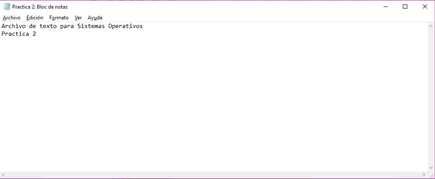
\includegraphics[scale=1.2]{Imagenes/Documentos/Archivotxt.png}
     
        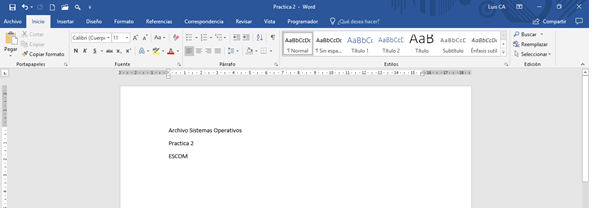
\includegraphics[scale=1.1]{Imagenes/Documentos/Archivoword.png}
     
        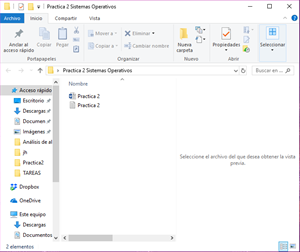
\includegraphics[scale=1.2]{Imagenes/Documentos/CarpetaDoc.png}
     \end{center}
    2.-Se inicia sesion en Linux
    
    3.-Se monta la memoria USB
    
    4.-Editamos los archivos de texto txt y word:
    \begin{center}
        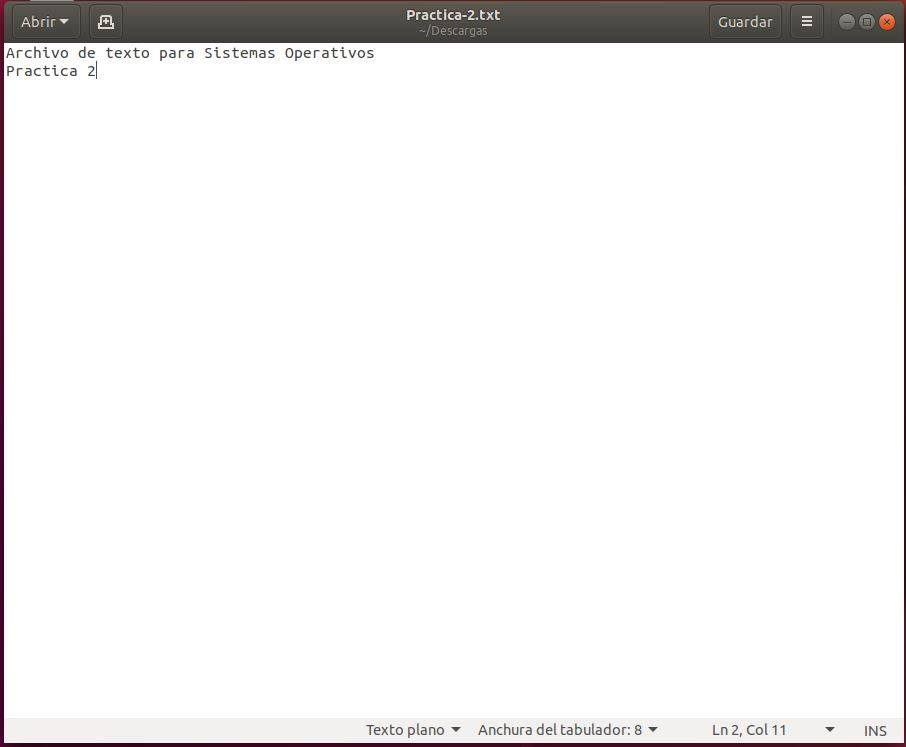
\includegraphics[scale=.3]{Imagenes/Documentos/41804851_314050915814812_2983270269323313152_n.jpg}
    
        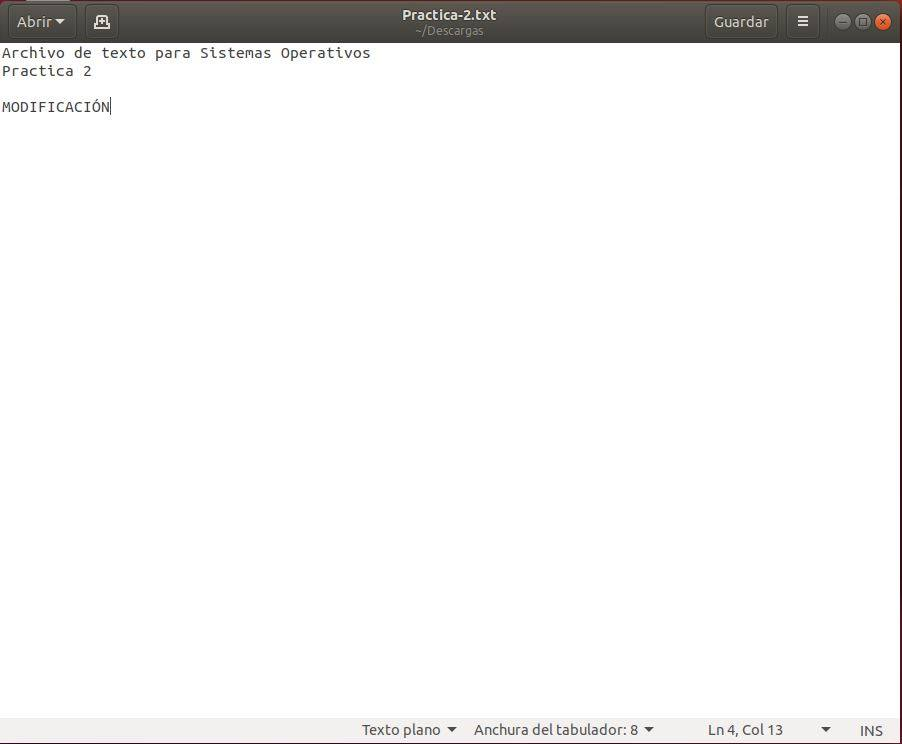
\includegraphics[scale=.3]{Imagenes/Documentos/41871764_911786172340337_107711659455283200_n.jpg}
    
        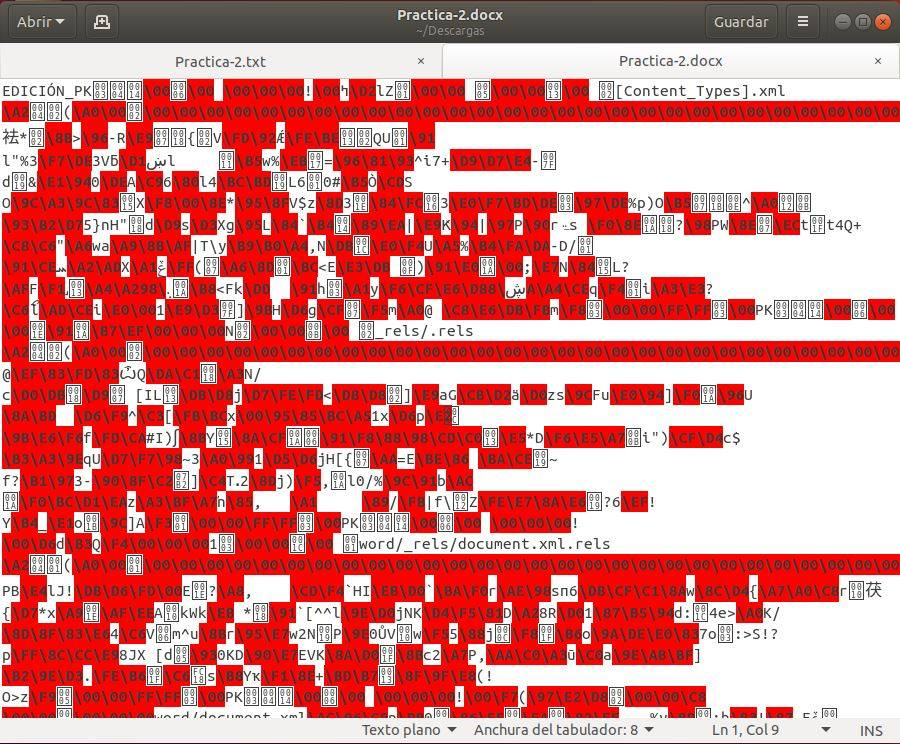
\includegraphics[scale=.3]{Imagenes/Documentos/41932670_956306477900580_2183251508575862784_n.jpg}
    
        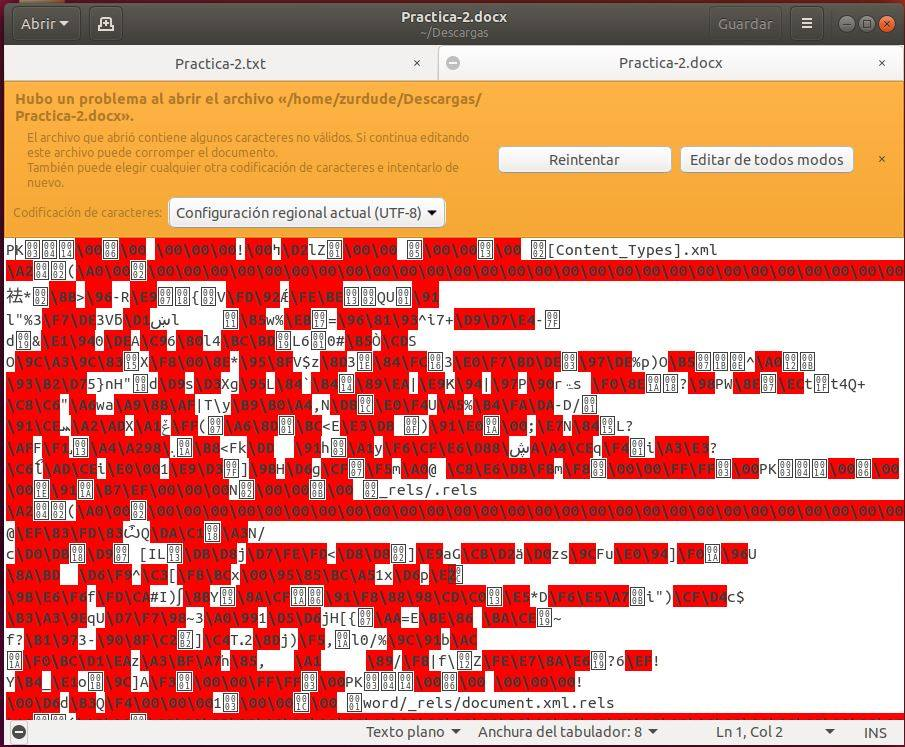
\includegraphics[scale=.3]{Imagenes/Documentos/41991608_2181774298735753_5343051968921206784_n.jpg}
    
    \end{center}
    
    5.-Abrimos los archivos de texto en Windows
    \begin{center}
        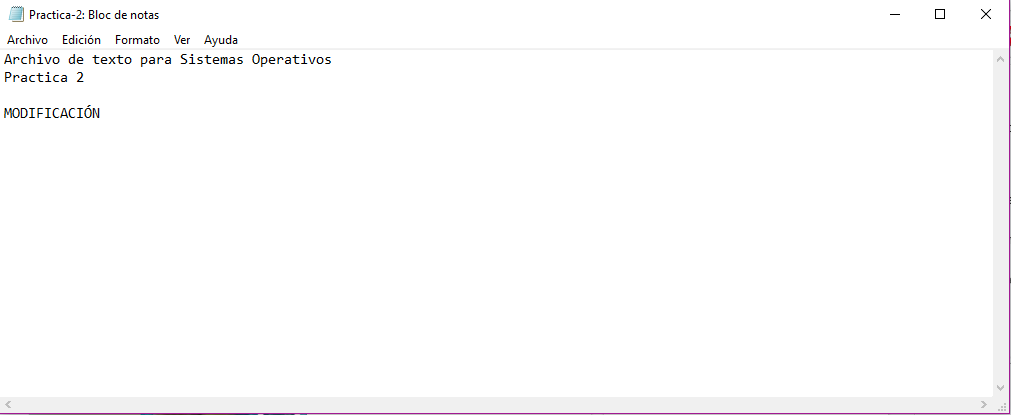
\includegraphics[scale=.4]{Imagenes/Documentos/Windowstxt.png}
        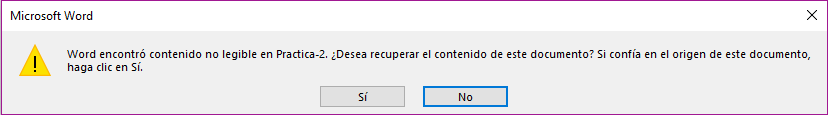
\includegraphics[scale=.6]{Imagenes/Documentos/Windowsword.png}
    \end{center}
    
    
    El archivo txt se ve bien, con todas las modificaciones que realizamos en Linux. Por otro lado, el archivo word no se pudo abrir; esto se debe a la diferencia de caracteres con los que trabajan.
    \newpage
    
\subsection{Llamadas al sistema en Linux.}
A continuación se explican las principales llamas del sistena Linux.

    \begin{tabular}{
			|p{5cm}|p{10cm}||}
			\hline
			\textbf{ Llamada al sistema.} & \textbf{ Descripción.}\\ 
			\hline
			\hline open & La llamada al sistema open () abre el archivo especificado por la ruta de acceso. Si el el archivo especificado no existe, puede opcionalmente  ser creado por open().
			El valor de retorno de open () es un descriptor de archivo, un número entero, no negativo, pequeño  que se usa en otras llamadas al sistema para referirse al archivo abierto.
			\\
			
			\hline close& Cambiar bits a modo de archivo.\\
			\hline read & Puede ser usado para editar todo tipo de texto sin formato. Es especialmente útil para editar programas.\\
			\hline write & La función write () intentará escribir n bytes desde el buffer señalado  al archivo asociado con el archivo abierto.\\
			\hline creat & Crea un nuevo archivo o reescribe uno existente. \\
			\hline lseek & Mover el desplazamiento de archivo de lectura / escritura.\\
			\hline access & Comprueba si el proceso de llamada puede acceder al nombre de ruta del archivo. Si el nombre de ruta del archivo es un enlace simbólico, se desreferencia.\\
			\hline stat & Devuelve información sobre un archivo. No se requieren permisos en el archivo en sí, pero en el caso de stat  se requiere permiso de ejecución (búsqueda) en todos los directorios en la ruta que conducen al archivo.\\
			\hline chmod & Cambia los permisos de un archivo \\
			\hline chown & Cambia de  propietario y grupo de archivos.\\
			\hline fcntl & Manipula el descriptor de archivo.\\
			\hline chdir & Cambia el directorio de trabajo.\\
			\hline mkdir & Crea un directorio.\\
			\hline opendir & Abrirá una secuencia de directorio correspondiente al directorio nombrado por el argumento\\
			\hline readdir & Leer un directorio.\\
			\hline
			\end{tabular}\\
			\newpage
			
A continuación se explican las principales llamas del sistena Windows.\\

			\begin{tabular}{
			|p{5cm}|p{10cm}||}
			\hline
			\textbf{ Llamada al sistema.} & \textbf{ Descripción.}\\ 
			\hline
			\hline OpenFile &Crea, abre, vuelve a abrir o elimina un archivo.Esta función tiene capacidades limitadas y no es recomendable.
			\\
			\hline CloseFile (CloseHandle)& Cierra un identificador de objeto abierto. Si un archivo está abierto cuando una aplicación finaliza, el sistema lo cierra automáticamente.\\
			\hline ReadFile & Lee datos del archivo o dispositivo de entrada / salida (E / S) especificado. Las lecturas se producen en la posición especificada por el puntero del archivo si el dispositivo lo admite. Esta función está diseñada para operaciones sincrónicas y asíncronas.\\
			\hline WriteFile & Escribe datos en el archivo o dispositivo de entrada / salida (E / S) especificado.Esta función está diseñada para operación síncrona y asíncrona.\\
			\hline CreateFile & Crea o abre un archivo o dispositivo de E / S. Los dispositivos de E / S utilizados más comúnmente son los siguientes: archivo, secuencia de archivos, directorio, disco físico, volumen, búfer de consola, unidad de cinta, recurso de comunicaciones, ranura de correo y tubería. La función devuelve un identificador que se puede utilizar para acceder al archivo o dispositivo para varios tipos de E / S según el archivo o dispositivo y las banderas y atributos especificados. \\
			\hline SetFilePointer &Mueve el puntero de archivo del archivo especificado. Esta función almacena el puntero del archivo en dos valores LONG.\\
			\hline CreateDirectory & Crea un nuevo directorio Si el sistema de archivos subyacente admite seguridad en archivos y directorios, la función aplica un descriptor de seguridad específico al nuevo directorio.\\
			\hline SetCurrentDirectory & Cambia el directorio actual para el proceso actual.\\
			\end{tabular}\\
			\newpage
			
A continuación se explican las principales funciones en Windows.\\
			
			 \begin{tabular}{
			|p{5cm}|p{10cm}||}
			\hline
			\textbf{ Función.} & \textbf{ Descripción.}\\ 
			\hline
			\hline stat & Obtiene el estado del archivo. La función stat () obtendrá información sobre el archivo nombrado. El argumento de ruta apunta a un nombre de ruta nombrando un archivo. No se requiere leer, escribir o ejecutar el permiso del archivo nombrado.
			\\
			\hline opendir& Abre un directorio. La función opendir () abrirá una secuencia de directorios correspondiente al directorio nombrado. \\
			\hline readir & Lee un directorio.  La función readdir () devolverá un puntero a una estructura que representa la entrada de directorio en la posición actual en la secuencia de directorio especificada por el argumento de dirección del directorio , y posicionará la secuencia de directorio en la entrada siguiente. Devolverá un puntero nulo al llegar al final de la secuencia de directorio. \\
			\hline 
			\end{tabular}\\
			
			La razón por la que no existe una llamada al sistema similar a chmod de Linux, la cúal modifica los permisos de un archivo, está dada por el Sistema de Archivos que maneja cada sistema operativo.
			
			Los sistemas UNIX o compatibles POSIX, incluyendo sistemas basados en Linux y Mac OS X, poseen un sistema simple para el manejo de permisos sobre archivos individuales. POSIX especifica también un sistema de listas de control de acceso (ACLs), pero sólo está implementado por ciertos sistemas de archivos y sistemas operativos. 
			
			Las variantes de DOS (incluyendo los productos de Microsoft MS-DOS, Windows 95, Windows 98, y Windows Me) no implementan ningún sistema de permisos. Existe un atributo de "solo lectura" y un atributo de "archivo oculto" que pueden ser asignados o quitados de cualquier archivo por cualquier usuario.
			
			Microsoft Windows NT y sus derivados (incluyendo Windows 2000 y Windows XP), así como VMS y OpenVMS usan listas de control de acceso (ACLs) para administrar un conjunto más complejo y variado de permisos.No tienen un atributo específico en el sistema de archivos que garantice su respectivo permiso de ejecución.
			
\newpage
\subsection{Programas Desarrollados}
    \begin{enumerate}
        \item Utilizando las llamadas al sistema revisasdas para Linux que sean necesarias, desarrolle un programa en C que cree una serie aleatoria de archivos (en una ruta especificada a través de una línea de comando, el directorio no debe existir previamente), el contenido de los archivos serán cadenas que estén almacenadas en un arreglo.
        \item Una vez creados los archivos con sus contenidos por el programa del punto 8 y utilizando las llamadas al sistema revisadas para Linux que sean necesarias, desarrolle un programa en C para cambiar los permisos de un archivo seleccionado por el usuario.
        \item Una vez creados los archivos con sus contenidos por el programa del punto 8 y utilizando las llamadas al sistema revisa para Linux que sean necesarias, desarrolle un programa en C que liste los archivos, creados mostrando su tamaño,fecha y hora de acceso.
        \item Una vez creados los archivos con sus contenidos por el programa del punto 8 y utilizando las llamadas al sistema revisa para Linux que sean necesarias,desarrolle un programa en C para mostrar el contenido de un archivo seleccionado por el usuario, y que copie uno o más de los archivos creados a un directorio previamente establecido.
        \item Desarrolle las versiones para Windows de los programas descritos en los punto 1,3 y 11, utilizando las llamdas al sistema revisadas para Windows que sean necesarias. 
    \end{enumerate}
    \subsubsection{Linux}
    \begin{itemize}
        \item \textbf{Creación de Archivos}\\
         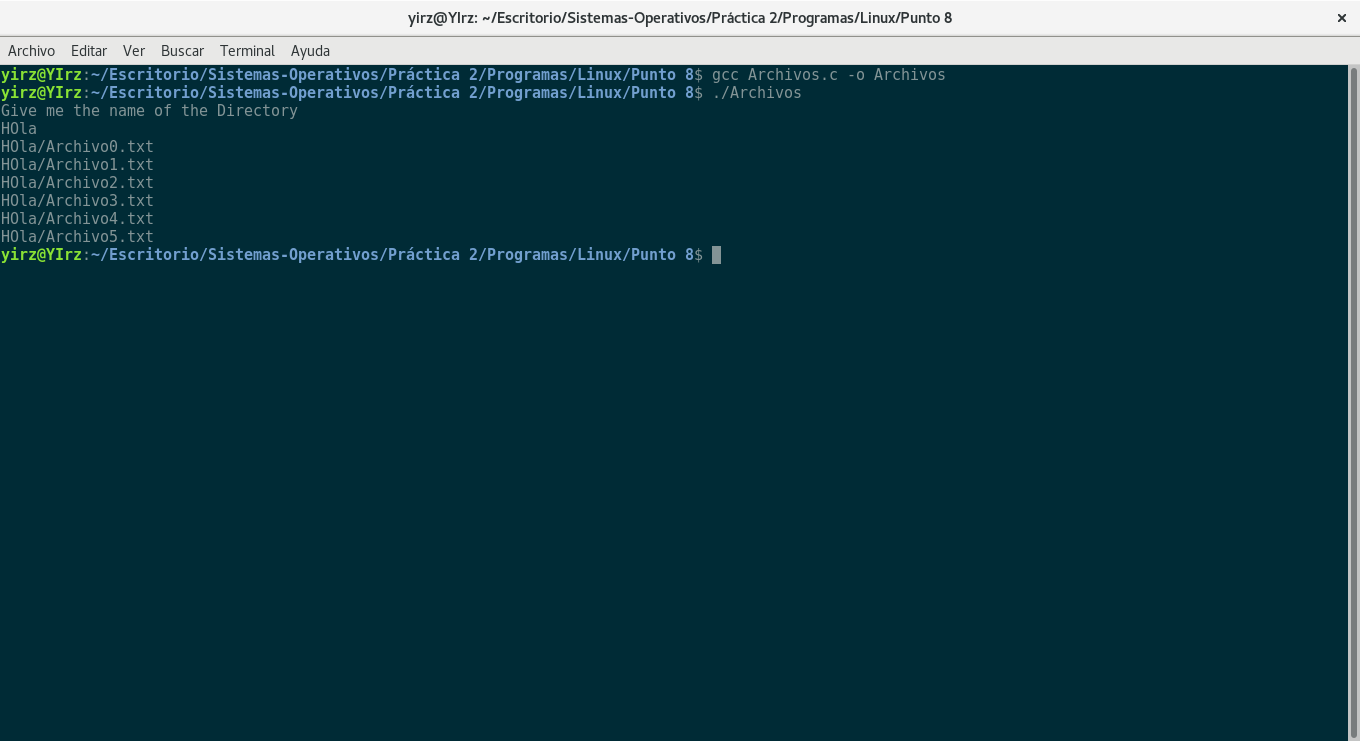
\includegraphics[scale=.3]{Imagenes/Linux/Archivos.png}\\
         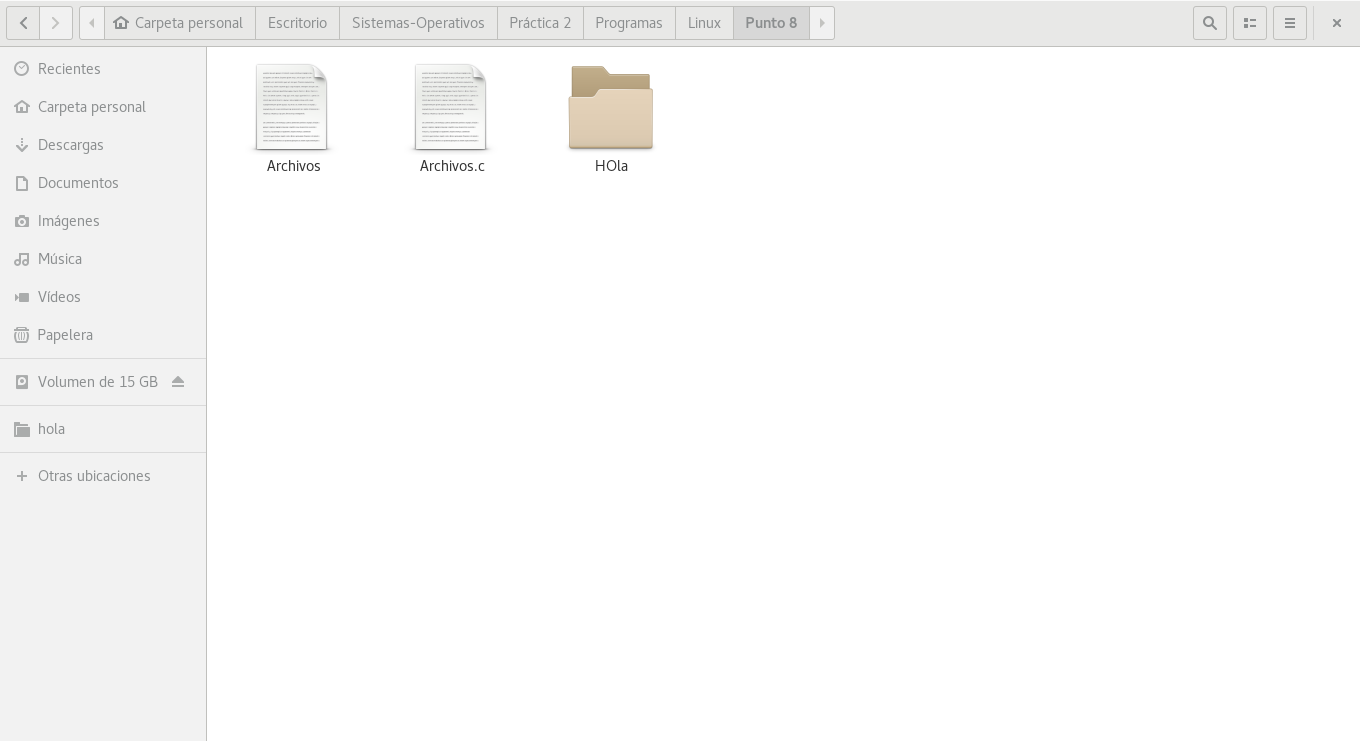
\includegraphics[scale=.3]{Imagenes/Linux/Archivos(1).png}\\
         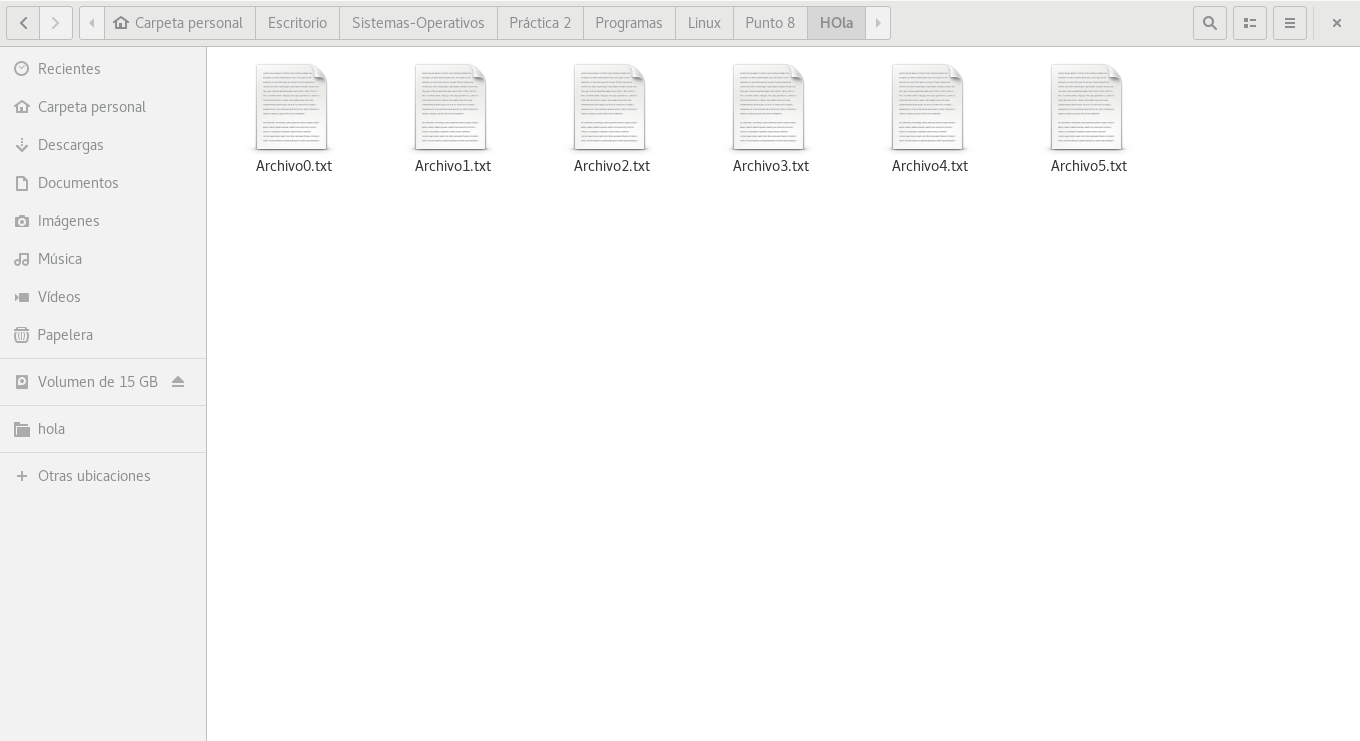
\includegraphics[scale=.3]{Imagenes/Linux/Archivos(2).png}\\
         \newpage
        \item \textbf{Cambio de permisos}\\
        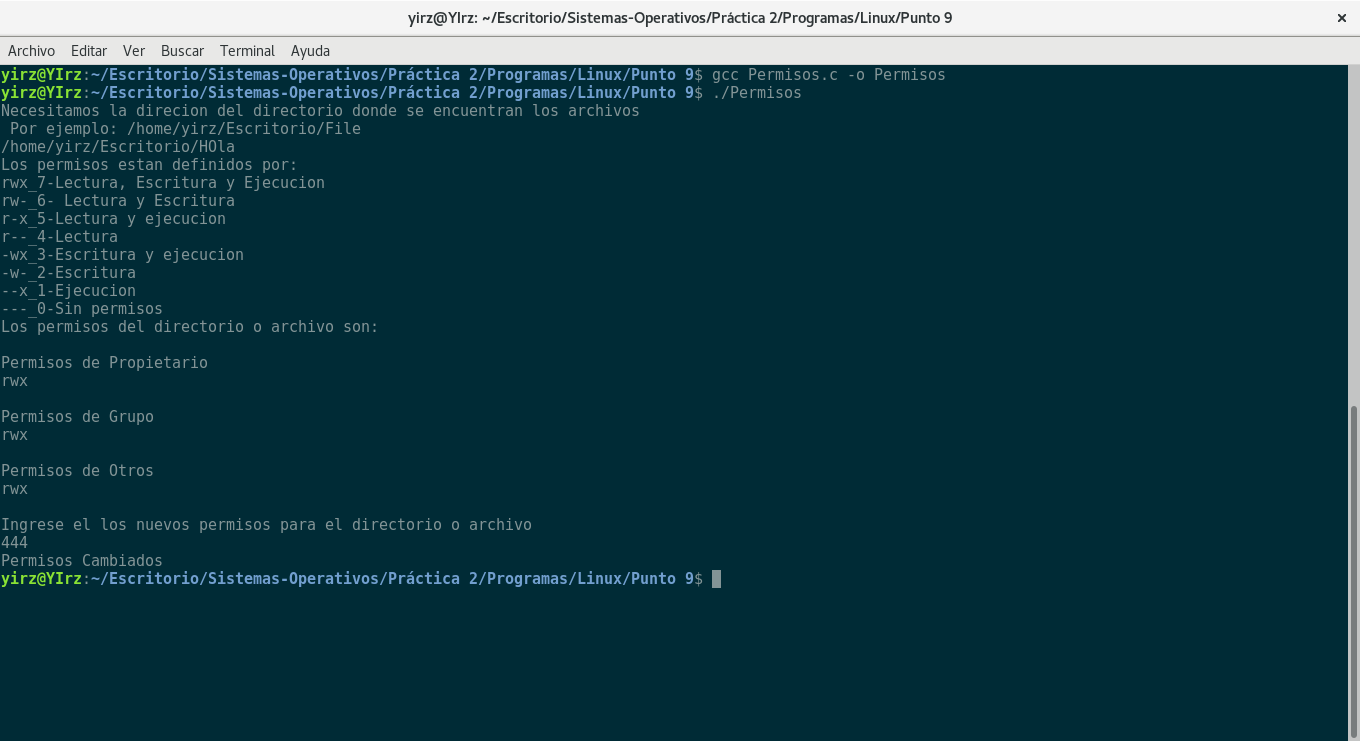
\includegraphics[scale=.3]{Imagenes/Linux/Permisos.png}\\
        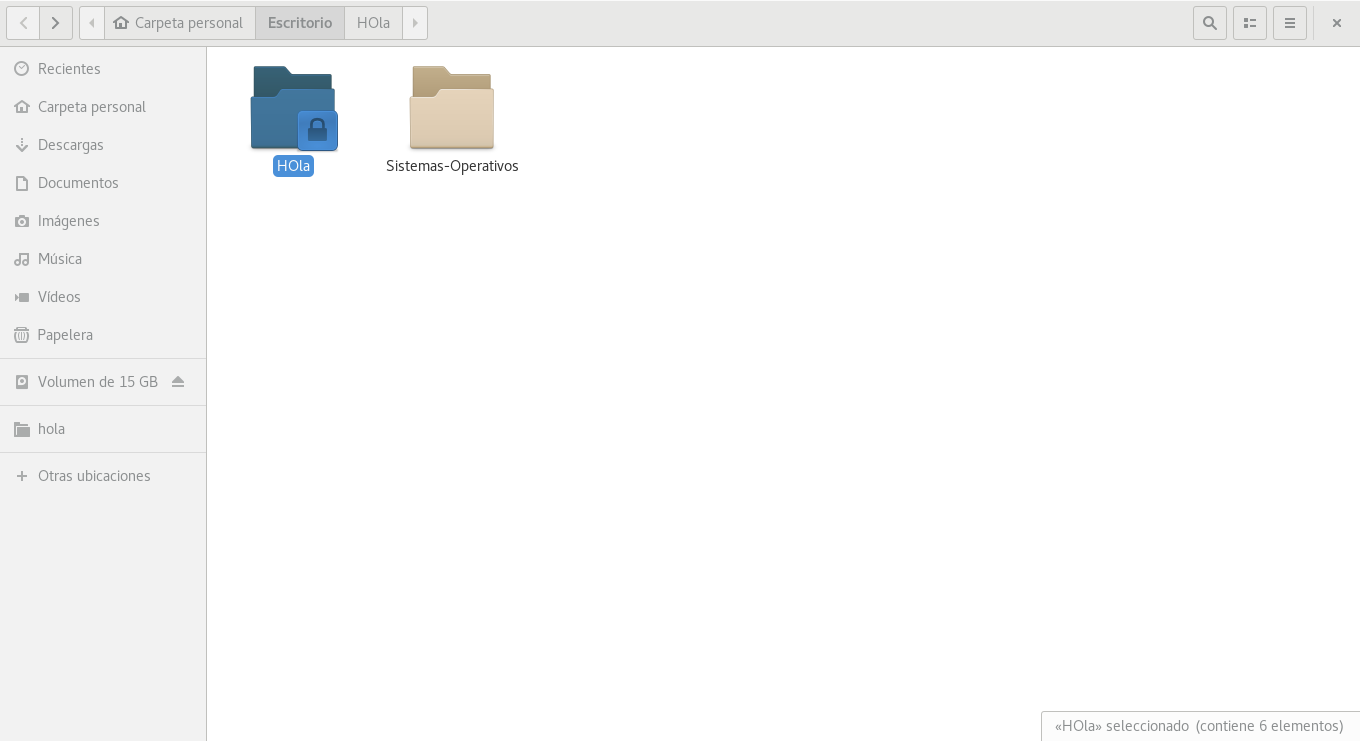
\includegraphics[scale=.3]{Imagenes/Linux/Permisos(1).png}\\
        \newpage
        \item  \textbf{ Enlistado de Archivos}\\
        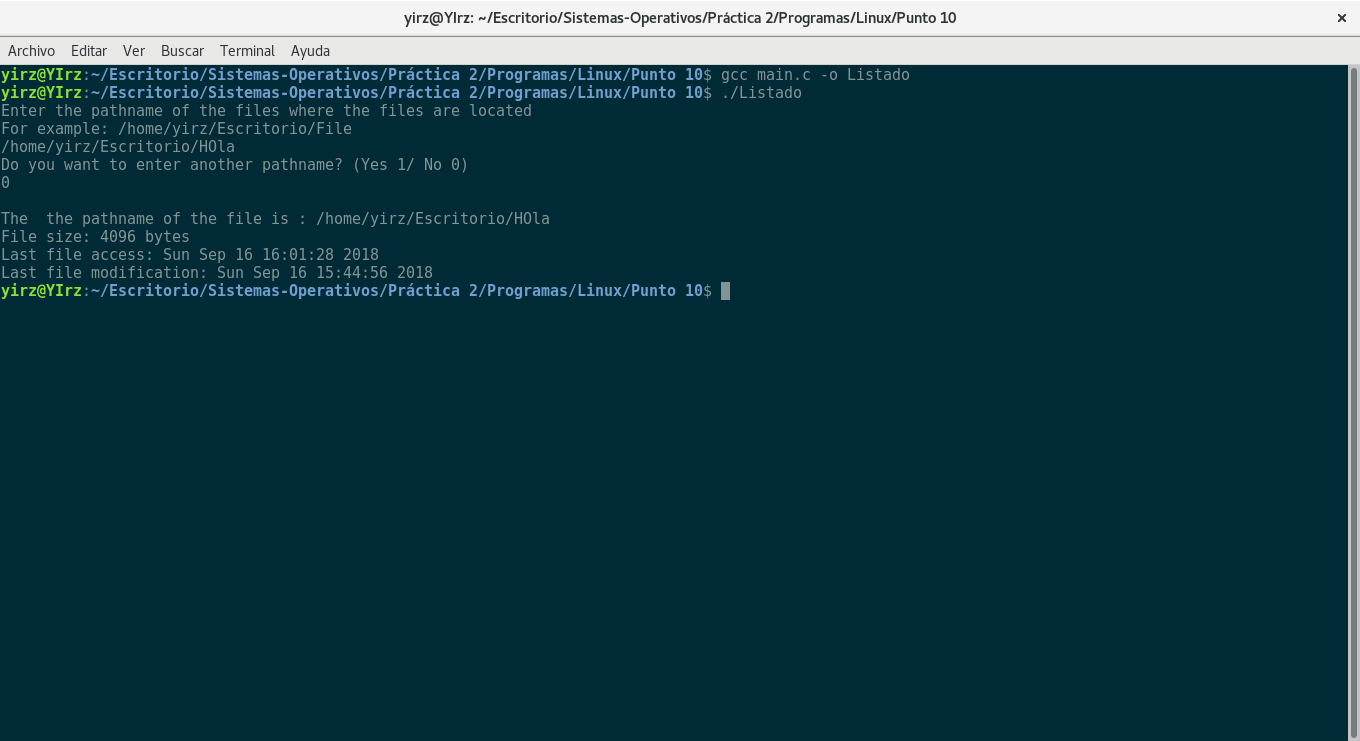
\includegraphics[scale=.3]{Imagenes/Linux/Listado.png}\\
        \item \textbf{Mostrar contenido de un archivo y copiado de archivos}\\
        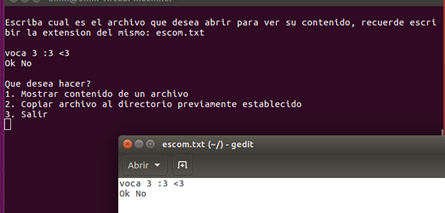
\includegraphics[scale=1.1]{Imagenes/Programa11/Prueba11L.png}\\
        
        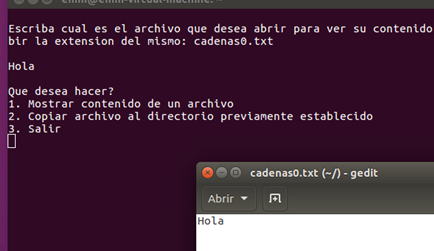
\includegraphics[scale=1.1]{Imagenes/Programa11/Prueba11L(1).png}\\
        
        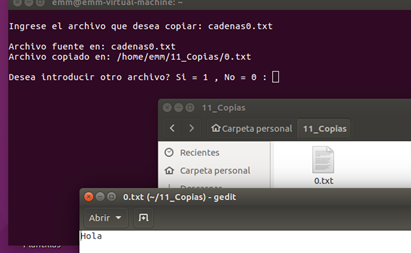
\includegraphics[scale=1.1]{Imagenes/Programa11/Prueba11L(2).png}\\
     
    \end{itemize}
     \subsubsection{Windows}
     \begin{itemize}
        \item \textbf{Creación de Archivos}\\
         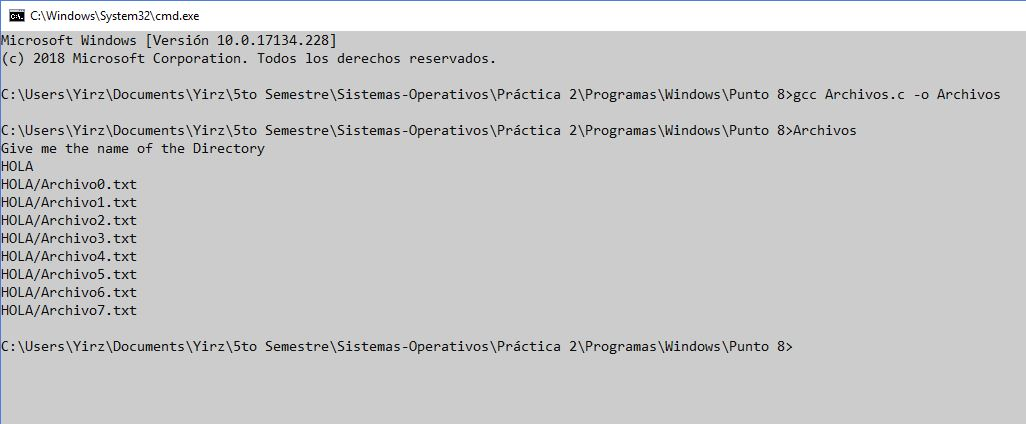
\includegraphics[scale=.5]{Imagenes/Windows/Archivos.png}\\
         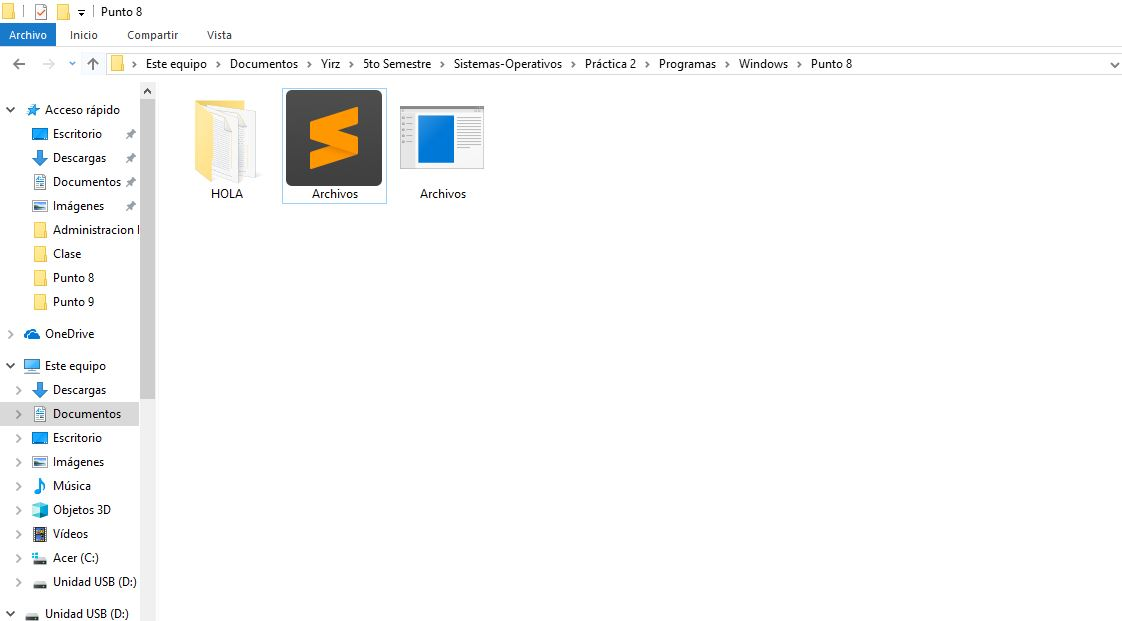
\includegraphics[scale=.5]{Imagenes/Windows/Archivos(1).png}\\
         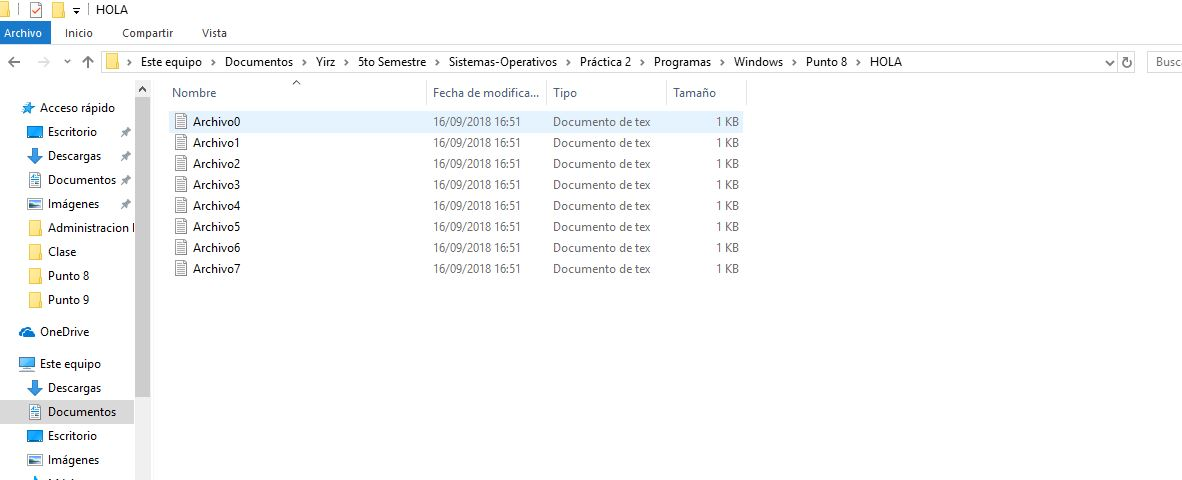
\includegraphics[scale=.5]{Imagenes/Windows/Archivos(2).png}\\
         \newpage
        \item  \textbf{ Enlistado de Archivos}\\
        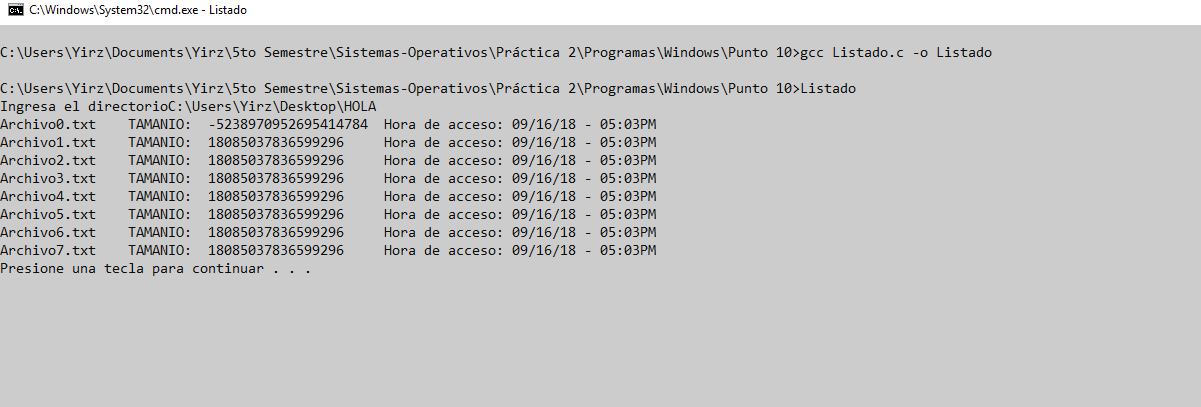
\includegraphics[scale=.5]{Imagenes/Windows/Listado.PNG}\\
        \item \textbf{Mostrar contenido de un archivo y copiado de archivos}\\
        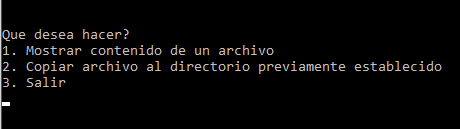
\includegraphics[scale=1.2]{Imagenes/Programa11/Prog11.png}
        
        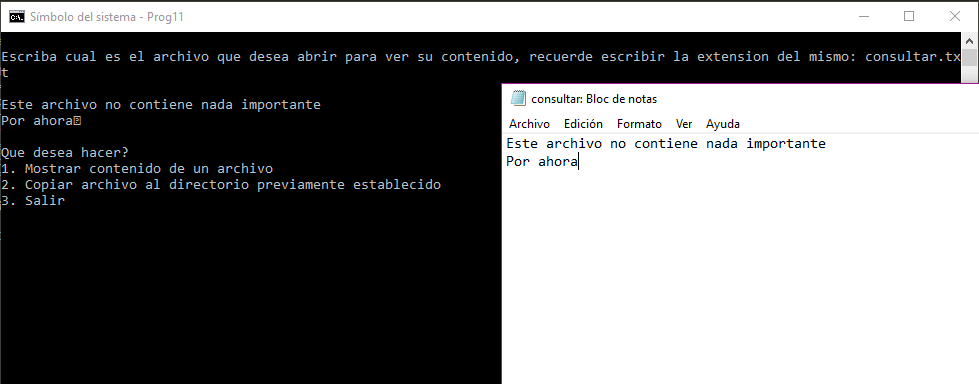
\includegraphics[scale=.7]{Imagenes/Programa11/Prog11prueba1.png}
        
        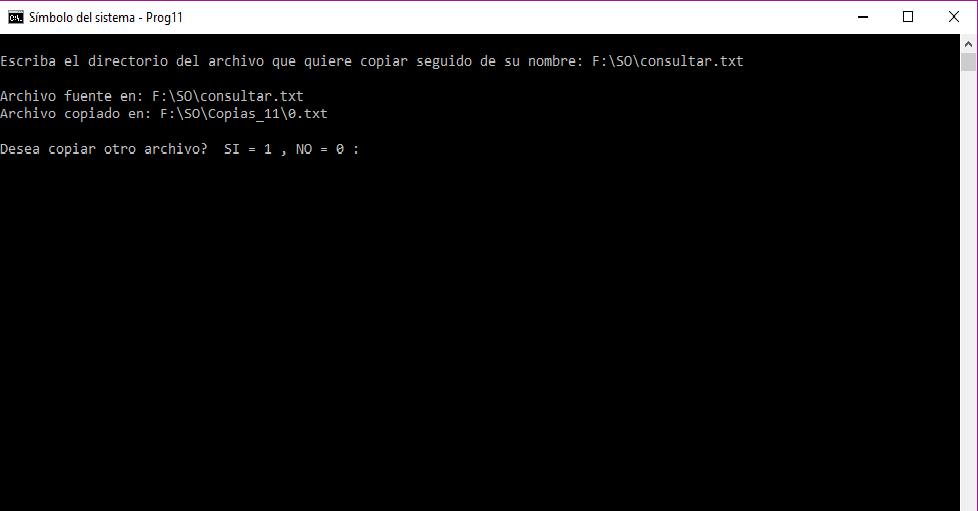
\includegraphics[scale=.7]{Imagenes/Programa11/Prog11Consultar1.png}
        
        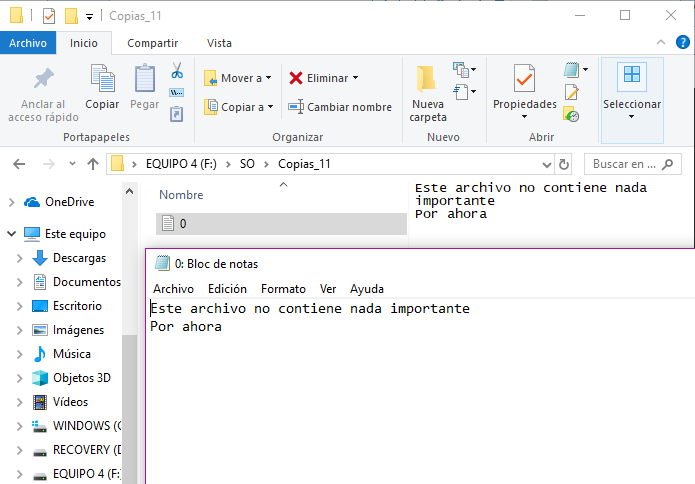
\includegraphics[scale=.7]{Imagenes/Programa11/Prog11Consultar2.png}
    \end{itemize}
    
    \newpage
\subsection{Código Fuente.}
    \subsubsection{Linux}
    Creación de Archivos
    \lstinputlisting{Codigo/Linux/Archivos.c}
    \newpage
    Cambio de permisos
    \lstinputlisting{Codigo/Linux/Permisos.c}
    Enlistado de Archivos
    \lstinputlisting{Codigo/Linux/main.c}
    Mostrar contenido de un archivo y copiado de archivos
    \lstinputlisting{Codigo/Linux/Prog11L.c}
    
            
    \subsubsection{Windows}
    Creación de Archivos
     \lstinputlisting{Codigo/Windows/Archivos.c}
     \newpage
     Enlistado de Archivos
     \lstinputlisting{Codigo/Windows/Listado.c}
     \newpage
     Mostrar contenido de un archivo y copiado de archivos
     \lstinputlisting{Codigo/Windows/Prog11.c}
     
     \newpage
\section{Observaciones.}

La principal observación que encontramos en el desarrollo de está práctica es la diferencia del tipo de sistema de archivos en los dos sistemas operativos, Linux y Windows, lo cual ocasiona que existan algunas diferencias entre la interacción con las interfaces de llamas al sistema entre los sistemas operativos, como fue el que el sistema operativo windows no permite un cambio en los permisos de usuario. 

Por otro lado, como sabemos las llamadas al sistema son la interfaz entre la capa de servicios y la capa de aplicación, por lo que al ser diferentes las llamas al sistema entre sistemas operativos en  consecuencia son diferentes los servicios o la forma en que se interactúa en la capa de aplicación.
\section{Análisis Crítico.}
Ambos sistemas operativos manejan llamadas a su sistema que nos permiten un acercamiento más profundo, íntimo vaya, al funcionamiento de cada sistema mediante comandos de cada uno, con los cuales pudimos manejar archivos (crearlos, escribir en ellos, obtener información, etc. ); sin embargo, es desde linux donde se tiene más libertad de utilizar este tipo de comandos, donde hay mayor diversidad de ellos, puesto que por naturaleza está diseñado para usuarios expertos en la utilización de un equipo de cómputo, ya que en windows algunas funcionalidades están en desuso o cuesta más trabajo implementarlas; en pocas palabras existe mayor restricción sobre el manejo de los archivos desde windows.
\section{Conclusiones.}
Se han cumplido los objetivos de esta práctica debido a que se implementaron con éxito las distintas llamadas al sistemas, tanto en linux como en windows, familiarizándonos con el uso de la interfaz de comandos respectiva. Hemos creado otra perspectiva sobre la funcionalidad de los sistemas operativos, manejando archivos como quizá pocos usuarios lo hayan experimentado, ya que las llamadas al sistemas nos permiten un control más íntimo de los archivos (de la información almacenada en un equipo de cómputo), siendo linux donde existe mayor control que en windows.
\end{document}
